\documentclass[a4paper]{book}
\usepackage{a4wide}
\usepackage{makeidx}
\usepackage{graphicx}
\usepackage{multicol}
\usepackage{float}
\usepackage{listings}
\usepackage{color}
\usepackage{textcomp}
\usepackage{alltt}
\usepackage{times}
\usepackage{ifpdf}
\ifpdf
\usepackage[pdftex,
            pagebackref=true,
            colorlinks=true,
            linkcolor=blue,
            unicode
           ]{hyperref}
\else
\usepackage[ps2pdf,
            pagebackref=true,
            colorlinks=true,
            linkcolor=blue,
            unicode
           ]{hyperref}
\usepackage{pspicture}
\fi
\usepackage[utf8]{inputenc}
\usepackage{doxygen}
\lstset{language=C++,inputencoding=utf8,basicstyle=\footnotesize,breaklines=true,breakatwhitespace=true,tabsize=8,numbers=left }
\makeindex
\setcounter{tocdepth}{3}
\renewcommand{\footrulewidth}{0.4pt}
\begin{document}
\hypersetup{pageanchor=false}
\begin{titlepage}
\vspace*{7cm}
\begin{center}
{\Large IMAR-\/C \\[1ex]\large 0.1 }\\
\vspace*{1cm}
{\large Generated by Doxygen 1.6.3}\\
\vspace*{0.5cm}
{\small Mon Jul 15 21:35:52 2013}\\
\end{center}
\end{titlepage}
\clearemptydoublepage
\pagenumbering{roman}
\tableofcontents
\clearemptydoublepage
\pagenumbering{arabic}
\hypersetup{pageanchor=true}
\chapter{File Index}
\section{File List}
Here is a list of all documented files with brief descriptions:\begin{DoxyCompactList}
\item\contentsline{section}{/home/noox/Documentos/programmation/c++/IMAR-\/C/src/{\bfseries denseTrack.cpp} }{\pageref{dense_track_8cpp}}{}
\item\contentsline{section}{/home/noox/Documentos/programmation/c++/IMAR-\/C/src/{\bfseries integration.cpp} }{\pageref{integration_8cpp}}{}
\item\contentsline{section}{/home/noox/Documentos/programmation/c++/IMAR-\/C/src/{\bfseries IplImagePyramid.cpp} }{\pageref{_ipl_image_pyramid_8cpp}}{}
\item\contentsline{section}{/home/noox/Documentos/programmation/c++/IMAR-\/C/src/{\bfseries IplImageWrapper.cpp} }{\pageref{_ipl_image_wrapper_8cpp}}{}
\item\contentsline{section}{/home/noox/Documentos/programmation/c++/IMAR-\/C/src/\hyperlink{naodensetrack_8cpp}{naodensetrack.cpp} (Set of function permiting to extract dense points and their trajectories )}{\pageref{naodensetrack_8cpp}}{}
\item\contentsline{section}{/home/noox/Documentos/programmation/c++/IMAR-\/C/src/\hyperlink{naokmeans_8cpp}{naokmeans.cpp} (Set of functions permiting to execute KMeans algorithms using KMlocal classes )}{\pageref{naokmeans_8cpp}}{}
\item\contentsline{section}{/home/noox/Documentos/programmation/c++/IMAR-\/C/src/{\bfseries naomngt.cpp} }{\pageref{naomngt_8cpp}}{}
\item\contentsline{section}{/home/noox/Documentos/programmation/c++/IMAR-\/C/src/\hyperlink{naosvm_8cpp}{naosvm.cpp} (Set of functions permiting to import/ predict a svm problem, import/create a svm model )}{\pageref{naosvm_8cpp}}{}
\item\contentsline{section}{/home/noox/Documentos/programmation/c++/IMAR-\/C/src/{\bfseries tactil.cpp} }{\pageref{tactil_8cpp}}{}
\item\contentsline{section}{/home/noox/Documentos/programmation/c++/IMAR-\/C/src/{\bfseries test.cpp} }{\pageref{test_8cpp}}{}
\end{DoxyCompactList}

\chapter{File Documentation}
\hypertarget{naodensetrack_8cpp}{
\section{naodensetrack.cpp File Reference}
\label{naodensetrack_8cpp}\index{naodensetrack.cpp@{naodensetrack.cpp}}
}


Set of function permiting to extract dense points and their trajectories.  


{\ttfamily \#include \char`\"{}naodensetrack.h\char`\"{}}\par
\subsection*{Functions}
\begin{DoxyCompactItemize}
\item 
\hypertarget{naodensetrack_8cpp_a226c48afad848525f02da428add19c14}{
CvScalar {\bfseries getRect} (const CvPoint2D32f point, const CvSize size, const DescInfo descInfo)}
\label{naodensetrack_8cpp_a226c48afad848525f02da428add19c14}

\item 
\hypertarget{naodensetrack_8cpp_a2e7ee2507f1a474d3dc994fd729dc97c}{
void {\bfseries BuildDescMat} (const IplImage $\ast$xComp, const IplImage $\ast$yComp, DescMat $\ast$descMat, const DescInfo descInfo)}
\label{naodensetrack_8cpp_a2e7ee2507f1a474d3dc994fd729dc97c}

\item 
\hypertarget{naodensetrack_8cpp_a7dea7a2ef95bb615663fb1425ed1be7f}{
std::vector$<$ float $>$ {\bfseries getDesc} (const DescMat $\ast$descMat, CvScalar rect, DescInfo descInfo, float epsilon)}
\label{naodensetrack_8cpp_a7dea7a2ef95bb615663fb1425ed1be7f}

\item 
\hypertarget{naodensetrack_8cpp_aa336a0d7bb1b157909f359e0755fbd46}{
void {\bfseries HogComp} (IplImage $\ast$img, DescMat $\ast$descMat, DescInfo descInfo)}
\label{naodensetrack_8cpp_aa336a0d7bb1b157909f359e0755fbd46}

\item 
\hypertarget{naodensetrack_8cpp_afd28d0706af758eedd32b62ba0e74d5b}{
void {\bfseries HofComp} (IplImage $\ast$flow, DescMat $\ast$descMat, DescInfo descInfo)}
\label{naodensetrack_8cpp_afd28d0706af758eedd32b62ba0e74d5b}

\item 
\hypertarget{naodensetrack_8cpp_a293d8b6ca474b2b9db95a5fca340d36a}{
void {\bfseries MbhComp} (IplImage $\ast$flow, DescMat $\ast$descMatX, DescMat $\ast$descMatY, DescInfo descInfo)}
\label{naodensetrack_8cpp_a293d8b6ca474b2b9db95a5fca340d36a}

\item 
\hypertarget{naodensetrack_8cpp_a3c4ede6cb74094c5ed25a847fe2a84a5}{
void {\bfseries OpticalFlowTracker} (IplImage $\ast$flow, std::vector$<$ CvPoint2D32f $>$ \&points\_\-in, std::vector$<$ CvPoint2D32f $>$ \&points\_\-out, std::vector$<$ int $>$ \&status)}
\label{naodensetrack_8cpp_a3c4ede6cb74094c5ed25a847fe2a84a5}

\item 
\hypertarget{naodensetrack_8cpp_ad3cd1ba8d80c4d87b1af9ee125c0f856}{
int {\bfseries isValid} (std::vector$<$ CvPoint2D32f $>$ \&track, float \&mean\_\-x, float \&mean\_\-y, float \&var\_\-x, float \&var\_\-y, float \&length, float min\_\-var, float max\_\-var, float max\_\-dis)}
\label{naodensetrack_8cpp_ad3cd1ba8d80c4d87b1af9ee125c0f856}

\item 
\hypertarget{naodensetrack_8cpp_a9125f8b77f4100c1e9b759cba36501c2}{
void {\bfseries cvDenseSample} (IplImage $\ast$grey, IplImage $\ast$eig, std::vector$<$ CvPoint2D32f $>$ \&points, const double quality, const double min\_\-distance)}
\label{naodensetrack_8cpp_a9125f8b77f4100c1e9b759cba36501c2}

\item 
\hypertarget{naodensetrack_8cpp_a8a65b2c7d216ab828100d9d1bfcc80c4}{
void {\bfseries cvDenseSample} (IplImage $\ast$grey, IplImage $\ast$eig, std::vector$<$ CvPoint2D32f $>$ \&points\_\-in, std::vector$<$ CvPoint2D32f $>$ \&points\_\-out, const double quality, const double min\_\-distance)}
\label{naodensetrack_8cpp_a8a65b2c7d216ab828100d9d1bfcc80c4}

\item 
\hypertarget{naodensetrack_8cpp_a96eff71ad3285b07f2ff23e92ebd61f5}{
void {\bfseries InitTrackerInfo} (TrackerInfo $\ast$tracker, int track\_\-length, int init\_\-gap)}
\label{naodensetrack_8cpp_a96eff71ad3285b07f2ff23e92ebd61f5}

\item 
\hypertarget{naodensetrack_8cpp_a6736ed6f2e97c2426473de79d658b6e6}{
DescMat $\ast$ {\bfseries InitDescMat} (int height, int width, int nBins)}
\label{naodensetrack_8cpp_a6736ed6f2e97c2426473de79d658b6e6}

\item 
\hypertarget{naodensetrack_8cpp_a41f252789efef14d9448d73ee73986b2}{
void {\bfseries ReleDescMat} (DescMat $\ast$descMat)}
\label{naodensetrack_8cpp_a41f252789efef14d9448d73ee73986b2}

\item 
\hypertarget{naodensetrack_8cpp_aaa264710c19b3eaab47ff882844da6f8}{
void {\bfseries InitDescInfo} (DescInfo $\ast$descInfo, int nBins, int flag, int orientation, int size, int nxy\_\-cell, int nt\_\-cell, float min\_\-flow)}
\label{naodensetrack_8cpp_aaa264710c19b3eaab47ff882844da6f8}

\item 
\hypertarget{naodensetrack_8cpp_a2ef30c42cbc289d899a8be5d2d8f77d0}{
void {\bfseries usage} ()}
\label{naodensetrack_8cpp_a2ef30c42cbc289d899a8be5d2d8f77d0}

\item 
int \hyperlink{naodensetrack_8cpp_a68a8241c68f51463e79a24a27014ec2e}{extractSTIPs} (std::string video, int dim, int maxPts, KMdata $\ast$dataPts)
\begin{DoxyCompactList}\small\item\em Permits to extract STIPs from a video .avi. It save the HOG and HOG of the trajectories in the object KMdata. \item\end{DoxyCompactList}\end{DoxyCompactItemize}


\subsection{Detailed Description}
Set of function permiting to extract dense points and their trajectories. \begin{DoxyAuthor}{Author}
LEAR 
\end{DoxyAuthor}
\begin{DoxyDate}{Date}
05/07/2013 
\end{DoxyDate}


Definition in file \hyperlink{naodensetrack_8cpp_source}{naodensetrack.cpp}.



\subsection{Function Documentation}
\hypertarget{naodensetrack_8cpp_a68a8241c68f51463e79a24a27014ec2e}{
\index{naodensetrack.cpp@{naodensetrack.cpp}!extractSTIPs@{extractSTIPs}}
\index{extractSTIPs@{extractSTIPs}!naodensetrack.cpp@{naodensetrack.cpp}}
\subsubsection[{extractSTIPs}]{\setlength{\rightskip}{0pt plus 5cm}int extractSTIPs (std::string {\em video}, \/  int {\em dim}, \/  int {\em maxPts}, \/  KMdata $\ast$ {\em dataPts})}}
\label{naodensetrack_8cpp_a68a8241c68f51463e79a24a27014ec2e}


Permits to extract STIPs from a video .avi. It save the HOG and HOG of the trajectories in the object KMdata. 


\begin{DoxyParams}{Parameters}
\item[\mbox{$\leftarrow$} {\em stip}]Name of the video. \item[\mbox{$\leftarrow$} {\em dim}]STIPs dimension. \item[\mbox{$\leftarrow$} {\em maxPts}]Maximum number of points we want to use. \item[\mbox{$\rightarrow$} {\em dataPts}]The object in which we save the STIPs. \end{DoxyParams}
\begin{DoxyReturn}{Returns}
Number of points extracted. 
\end{DoxyReturn}


Definition at line 491 of file naodensetrack.cpp.


\hypertarget{naokmeans_8cpp}{
\section{/home/noox/Documentos/programmation/c++/IMAR-\/C/src/naokmeans.cpp File Reference}
\label{naokmeans_8cpp}\index{/home/noox/Documentos/programmation/c++/IMAR-\/C/src/naokmeans.cpp@{/home/noox/Documentos/programmation/c++/IMAR-\/C/src/naokmeans.cpp}}
}


Set of functions permiting to execute KMeans algorithms using KMlocal classes.  


{\ttfamily \#include \char`\"{}naokmeans.h\char`\"{}}\par
{\ttfamily \#include $<$time.h$>$}\par
Include dependency graph for naokmeans.cpp:\nopagebreak
\begin{figure}[H]
\begin{center}
\leavevmode
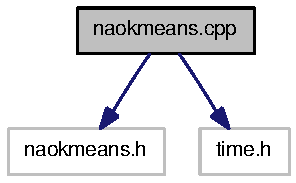
\includegraphics[width=191pt]{naokmeans_8cpp__incl}
\end{center}
\end{figure}
\subsection*{Functions}
\begin{DoxyCompactItemize}
\item 
int \hyperlink{naokmeans_8cpp_a4a594810a9a736a792e6b2571dfc2170}{importSTIPs} (std::string stip, int dim, int maxPts, KMdata $\ast$dataPts)
\begin{DoxyCompactList}\small\item\em STIPs importation function in the format 1 point = 1 line. Each dimension are separated from one space (\char`\"{} \char`\"{}). \item\end{DoxyCompactList}\item 
\hypertarget{naokmeans_8cpp_a78f6f33e72a52c581dfd286a3920f6bf}{
void {\bfseries exportSTIPs} (std::string stip, int dim, const KMdata \&dataPts)}
\label{naokmeans_8cpp_a78f6f33e72a52c581dfd286a3920f6bf}

\item 
void \hyperlink{naokmeans_8cpp_a70fee2c407d3bf32b07943b8cfcb3c7e}{exportCenters} (std::string centers, int dim, int k, KMfilterCenters ctrs)
\begin{DoxyCompactList}\small\item\em Export function to save KMfilterCenters in a file. One line corresponds to one point with dim value (separeted from one space \char`\"{} \char`\"{}). \item\end{DoxyCompactList}\item 
void \hyperlink{naokmeans_8cpp_ab24dc2206c891d1c5644ba930daa6e74}{importCenters} (std::string centers, int dim, int k, KMfilterCenters $\ast$ctrs)
\begin{DoxyCompactList}\small\item\em Importation function saving external centers in the KMfilterCenters object. One line corresponds to one centers with its values (separeted from one space \char`\"{} \char`\"{}). \item\end{DoxyCompactList}\item 
void \hyperlink{naokmeans_8cpp_a1239738af8b88f74abba7ca22baaf46c}{kmIvanAlgorithm} (int ic, int dim, const KMdata \&dataPts, int k, KMfilterCenters \&ctrs)
\begin{DoxyCompactList}\small\item\em This is an optimized KMeans algorithm. Ivan's algorithm uses basic KMeans algorithm (here the Lloyd's one) and the idea was to initialize centers intelligently. \item\end{DoxyCompactList}\end{DoxyCompactItemize}


\subsection{Detailed Description}
Set of functions permiting to execute KMeans algorithms using KMlocal classes. \begin{DoxyAuthor}{Author}
Fabien ROUALDES (institut Mines-\/Télécom) 
\end{DoxyAuthor}
\begin{DoxyDate}{Date}
02/07/2013 
\end{DoxyDate}


Definition in file \hyperlink{naokmeans_8cpp_source}{naokmeans.cpp}.



\subsection{Function Documentation}
\hypertarget{naokmeans_8cpp_a70fee2c407d3bf32b07943b8cfcb3c7e}{
\index{naokmeans.cpp@{naokmeans.cpp}!exportCenters@{exportCenters}}
\index{exportCenters@{exportCenters}!naokmeans.cpp@{naokmeans.cpp}}
\subsubsection[{exportCenters}]{\setlength{\rightskip}{0pt plus 5cm}void exportCenters (std::string {\em centers}, \/  int {\em dim}, \/  int {\em k}, \/  KMfilterCenters {\em ctrs})}}
\label{naokmeans_8cpp_a70fee2c407d3bf32b07943b8cfcb3c7e}


Export function to save KMfilterCenters in a file. One line corresponds to one point with dim value (separeted from one space \char`\"{} \char`\"{}). 


\begin{DoxyParams}{Parameters}
\item[\mbox{$\leftarrow$} {\em centers}]Name of the file which will be containing dimensions of each centers. \item[\mbox{$\leftarrow$} {\em dim}]Center's dimension. \item[\mbox{$\leftarrow$} {\em k}]Number of centers. \item[\mbox{$\leftarrow$} {\em ctrs}]The centers. \end{DoxyParams}


Definition at line 83 of file naokmeans.cpp.

\hypertarget{naokmeans_8cpp_ab24dc2206c891d1c5644ba930daa6e74}{
\index{naokmeans.cpp@{naokmeans.cpp}!importCenters@{importCenters}}
\index{importCenters@{importCenters}!naokmeans.cpp@{naokmeans.cpp}}
\subsubsection[{importCenters}]{\setlength{\rightskip}{0pt plus 5cm}void importCenters (std::string {\em centers}, \/  int {\em dim}, \/  int {\em k}, \/  KMfilterCenters $\ast$ {\em ctrs})}}
\label{naokmeans_8cpp_ab24dc2206c891d1c5644ba930daa6e74}


Importation function saving external centers in the KMfilterCenters object. One line corresponds to one centers with its values (separeted from one space \char`\"{} \char`\"{}). 


\begin{DoxyParams}{Parameters}
\item[\mbox{$\leftarrow$} {\em centers}]Name of the file which will be containing dimensions of each centers. \item[\mbox{$\leftarrow$} {\em dim}]Center's dimension. \item[\mbox{$\leftarrow$} {\em k}]Number of centers. \item[\mbox{$\rightarrow$} {\em ctrs}]The centers. \end{DoxyParams}


Definition at line 109 of file naokmeans.cpp.

\hypertarget{naokmeans_8cpp_a4a594810a9a736a792e6b2571dfc2170}{
\index{naokmeans.cpp@{naokmeans.cpp}!importSTIPs@{importSTIPs}}
\index{importSTIPs@{importSTIPs}!naokmeans.cpp@{naokmeans.cpp}}
\subsubsection[{importSTIPs}]{\setlength{\rightskip}{0pt plus 5cm}int importSTIPs (std::string {\em stip}, \/  int {\em dim}, \/  int {\em maxPts}, \/  KMdata $\ast$ {\em dataPts})}}
\label{naokmeans_8cpp_a4a594810a9a736a792e6b2571dfc2170}


STIPs importation function in the format 1 point = 1 line. Each dimension are separated from one space (\char`\"{} \char`\"{}). 


\begin{DoxyParams}{Parameters}
\item[\mbox{$\leftarrow$} {\em stip}]Name of the file containing the STIPs. \item[\mbox{$\leftarrow$} {\em dim}]The STIPs dimension. \item[\mbox{$\leftarrow$} {\em maxPts}]The maximum number of points you want to import. \item[\mbox{$\rightarrow$} {\em dataPts}]The KMlocal object which will be containing STIPs. \end{DoxyParams}
\begin{DoxyReturn}{Returns}
Number of points imported. 
\end{DoxyReturn}


Definition at line 23 of file naokmeans.cpp.

\hypertarget{naokmeans_8cpp_a1239738af8b88f74abba7ca22baaf46c}{
\index{naokmeans.cpp@{naokmeans.cpp}!kmIvanAlgorithm@{kmIvanAlgorithm}}
\index{kmIvanAlgorithm@{kmIvanAlgorithm}!naokmeans.cpp@{naokmeans.cpp}}
\subsubsection[{kmIvanAlgorithm}]{\setlength{\rightskip}{0pt plus 5cm}void kmIvanAlgorithm (int {\em ic}, \/  int {\em dim}, \/  const KMdata \& {\em dataPts}, \/  int {\em k}, \/  KMfilterCenters \& {\em ctrs})}}
\label{naokmeans_8cpp_a1239738af8b88f74abba7ca22baaf46c}


This is an optimized KMeans algorithm. Ivan's algorithm uses basic KMeans algorithm (here the Lloyd's one) and the idea was to initialize centers intelligently. 


\begin{DoxyParams}{Parameters}
\item[\mbox{$\leftarrow$} {\em ic}]The iteration coefficient will determine the number of iterations in each phases. \item[\mbox{$\leftarrow$} {\em dim}]Points and centers's dimension. \item[\mbox{$\leftarrow$} {\em dataPts}]The data we want to compute the centers. \item[\mbox{$\leftarrow$} {\em k}]The number of centers. \item[\mbox{$\rightarrow$} {\em ctrs}]The centers.\end{DoxyParams}
The Ivan's algorithm is divided into 3 phases. The first phase is executed on 25 per cent of the data (randomly sampled). To begin, the centers are randomly generated. Then ic $\ast$ 4 iterations of a KMeans algorithm are executed. During the second part we cluster 50 per cent of the data using the older centroids. This step is computed ic $\ast$ 2 times. Finally, we make ic $\ast$ 1 iteration on all the data. 

Definition at line 149 of file naokmeans.cpp.


\hypertarget{naosvm_8cpp}{
\section{naosvm.cpp File Reference}
\label{naosvm_8cpp}\index{naosvm.cpp@{naosvm.cpp}}
}


Set of functions permiting to import/ predict a svm problem, import/create a svm model.  


{\ttfamily \#include \char`\"{}naosvm.h\char`\"{}}\par
Include dependency graph for naosvm.cpp:\nopagebreak
\begin{figure}[H]
\begin{center}
\leavevmode
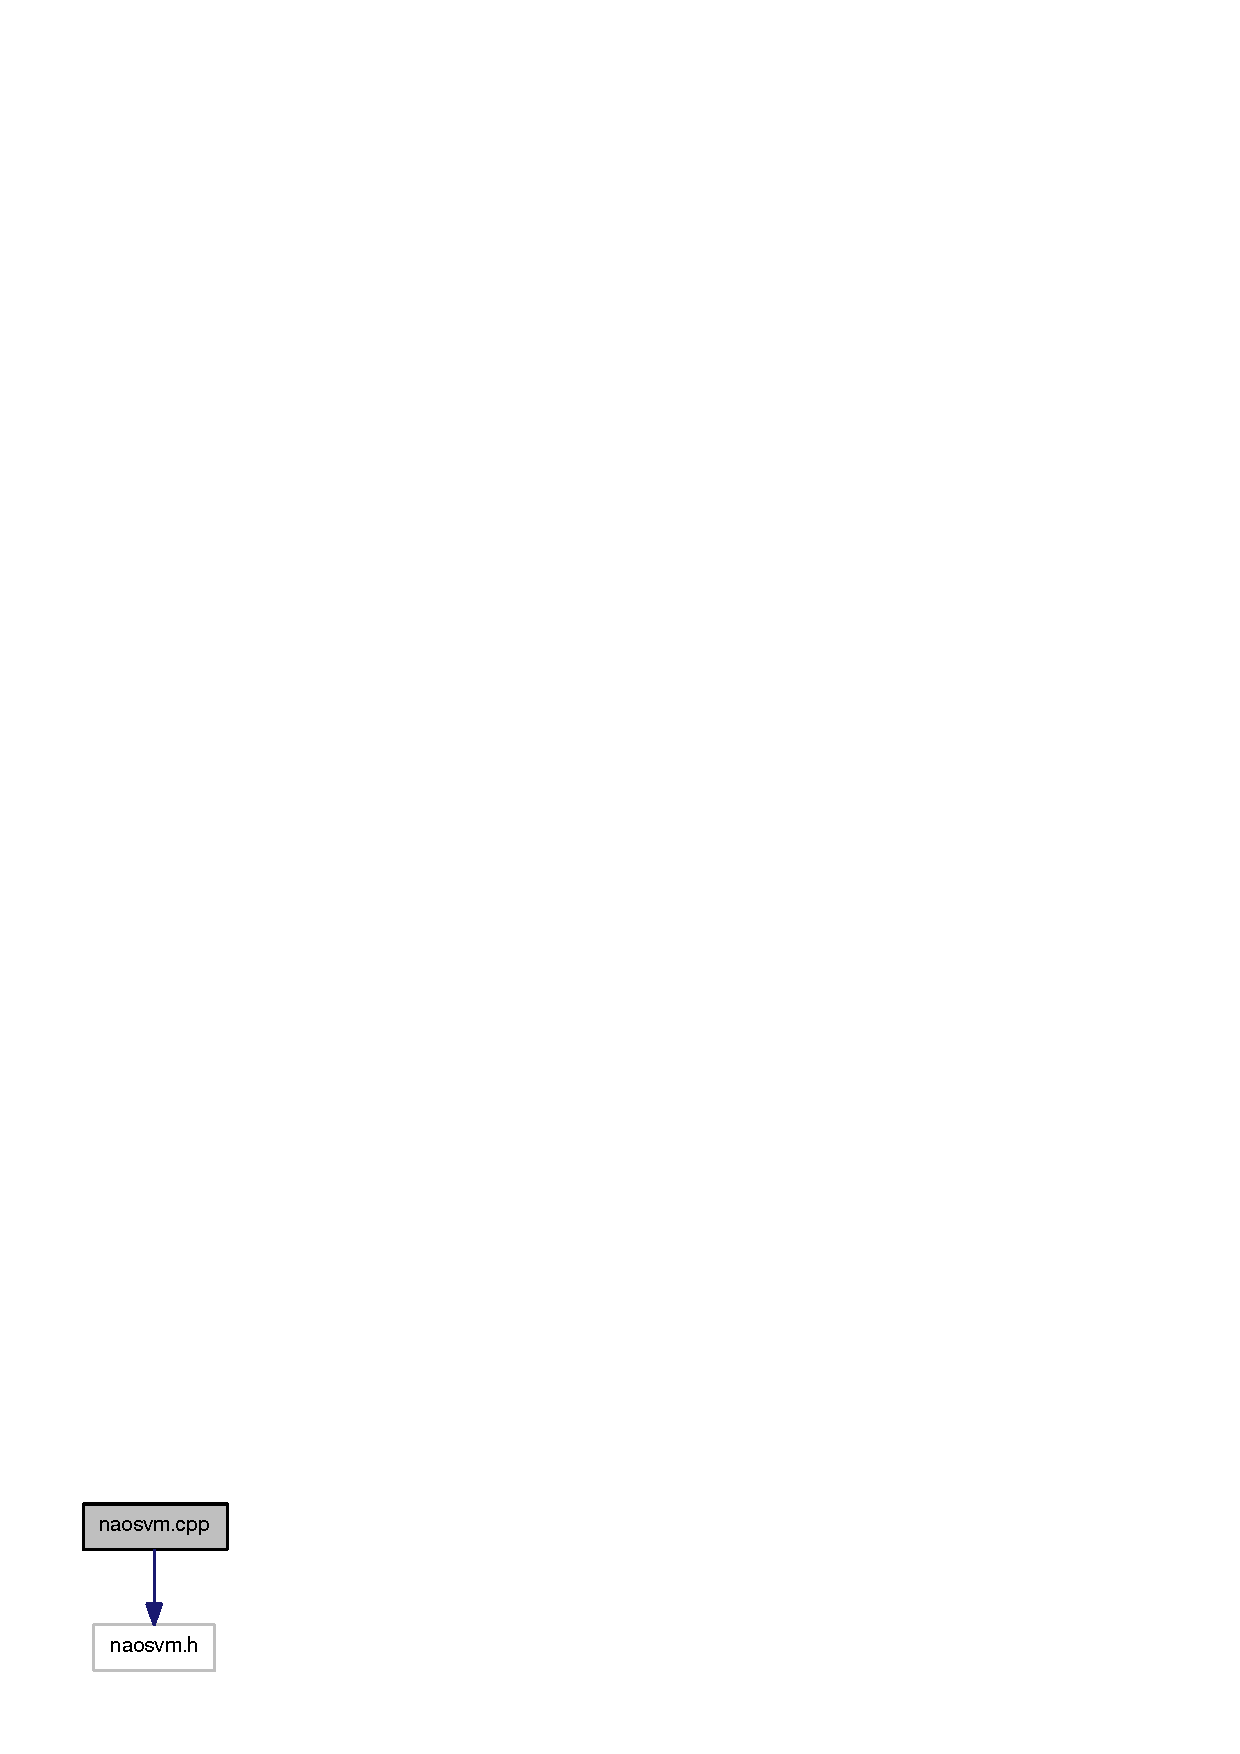
\includegraphics[width=56pt]{naosvm_8cpp__incl}
\end{center}
\end{figure}
\subsection*{Functions}
\begin{DoxyCompactItemize}
\item 
\hypertarget{naosvm_8cpp_a5313f9d3c2b41700153af19330e69de2}{
struct svm\_\-problem {\bfseries importProblem} (std::string file, int k)}
\label{naosvm_8cpp_a5313f9d3c2b41700153af19330e69de2}

\item 
\hypertarget{naosvm_8cpp_a906e1ea5bd8c8a6a5a2077ae804c0221}{
void {\bfseries exportProblem} (struct svm\_\-problem svmProblem, std::string file)}
\label{naosvm_8cpp_a906e1ea5bd8c8a6a5a2077ae804c0221}

\item 
\hypertarget{naosvm_8cpp_a7f0b66daba6744697b91575a3c328e4f}{
void {\bfseries exportProblemZero} (struct svm\_\-problem svmProblem, std::string file, int k)}
\label{naosvm_8cpp_a7f0b66daba6744697b91575a3c328e4f}

\item 
\hypertarget{naosvm_8cpp_a3c6544d006823a10250e0c9d14833945}{
struct svm\_\-problem {\bfseries computeBOW} (int label, const KMdata \&dataPts, KMfilterCenters \&ctrs)}
\label{naosvm_8cpp_a3c6544d006823a10250e0c9d14833945}

\item 
void \hyperlink{naosvm_8cpp_ada6d52e33a73b573605c6681a59cdacf}{printProblem} (struct svm\_\-problem svmProblem)
\begin{DoxyCompactList}\small\item\em It permits to print the SVM problem in the standard output. \item\end{DoxyCompactList}\item 
int \hyperlink{naosvm_8cpp_a2cae31212448e4bff07b0c79f0b1b592}{nrOfLines} (std::string filename)
\begin{DoxyCompactList}\small\item\em A function returning the number of lines (which correspond to the number of activities). \item\end{DoxyCompactList}\item 
void \hyperlink{naosvm_8cpp_a4c47d451dccceb9fbc24eb979ac87042}{printProbability} (struct svm\_\-model $\ast$pModel, struct svm\_\-node $\ast$nodes)
\begin{DoxyCompactList}\small\item\em Print for each labels the probability of the activity (stored in the SVM node structure). \item\end{DoxyCompactList}\item 
\hypertarget{naosvm_8cpp_a1e65e18e29d628fa8f395716eaebbf7c}{
struct svm\_\-model $\ast$ {\bfseries createSvmModel} (std::string bowFile, int k)}
\label{naosvm_8cpp_a1e65e18e29d628fa8f395716eaebbf7c}

\end{DoxyCompactItemize}


\subsection{Detailed Description}
Set of functions permiting to import/ predict a svm problem, import/create a svm model. \begin{DoxyAuthor}{Author}
Fabien ROUALDES (institut Mines-\/Télécom) 
\end{DoxyAuthor}
\begin{DoxyDate}{Date}
17/07/2013 
\end{DoxyDate}


Definition in file \hyperlink{naosvm_8cpp_source}{naosvm.cpp}.



\subsection{Function Documentation}
\hypertarget{naosvm_8cpp_a2cae31212448e4bff07b0c79f0b1b592}{
\index{naosvm.cpp@{naosvm.cpp}!nrOfLines@{nrOfLines}}
\index{nrOfLines@{nrOfLines}!naosvm.cpp@{naosvm.cpp}}
\subsubsection[{nrOfLines}]{\setlength{\rightskip}{0pt plus 5cm}int nrOfLines (std::string {\em filename})}}
\label{naosvm_8cpp_a2cae31212448e4bff07b0c79f0b1b592}


A function returning the number of lines (which correspond to the number of activities). 


\begin{DoxyParams}{Parameters}
\item[\mbox{$\leftarrow$} {\em fileName}]The file we want to count the number of lines. \end{DoxyParams}
\begin{DoxyReturn}{Returns}
The number of lines of the file. 
\end{DoxyReturn}


Definition at line 282 of file naosvm.cpp.

\hypertarget{naosvm_8cpp_a4c47d451dccceb9fbc24eb979ac87042}{
\index{naosvm.cpp@{naosvm.cpp}!printProbability@{printProbability}}
\index{printProbability@{printProbability}!naosvm.cpp@{naosvm.cpp}}
\subsubsection[{printProbability}]{\setlength{\rightskip}{0pt plus 5cm}void printProbability (struct svm\_\-model $\ast$ {\em pModel}, \/  struct svm\_\-node $\ast$ {\em nodes})}}
\label{naosvm_8cpp_a4c47d451dccceb9fbc24eb979ac87042}


Print for each labels the probability of the activity (stored in the SVM node structure). 


\begin{DoxyParams}{Parameters}
\item[\mbox{$\leftarrow$} {\em pModel}]A pointer to the SVM model. \item[\mbox{$\leftarrow$} {\em nodes}]The activity stored in SVM nodes. \end{DoxyParams}


Definition at line 304 of file naosvm.cpp.

\hypertarget{naosvm_8cpp_ada6d52e33a73b573605c6681a59cdacf}{
\index{naosvm.cpp@{naosvm.cpp}!printProblem@{printProblem}}
\index{printProblem@{printProblem}!naosvm.cpp@{naosvm.cpp}}
\subsubsection[{printProblem}]{\setlength{\rightskip}{0pt plus 5cm}void printProblem (struct svm\_\-problem {\em svmProblem})}}
\label{naosvm_8cpp_ada6d52e33a73b573605c6681a59cdacf}


It permits to print the SVM problem in the standard output. 


\begin{DoxyParams}{Parameters}
\item[\mbox{$\leftarrow$} {\em svmProblem}]It is the structure containing the SVM problem. \end{DoxyParams}


Definition at line 245 of file naosvm.cpp.


\printindex
\end{document}
